\begin{figure}
\centering
\subfloat{%
\begin{minipage}{0.40\textwidth}
   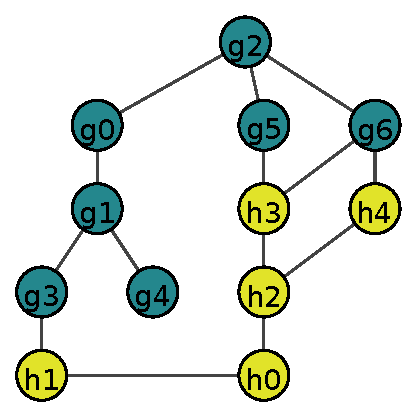
\includegraphics[width=0.8\textwidth]{figures/tiny_tree_graph}
\end{minipage}
}
\subfloat{%
\begin{minipage}{0.40\textwidth}

   \resizebox{\textwidth}{!}{%
      \begin{tabular}{@{}ll@{}}
         \toprule
         \textbf{moment}      & \textbf{quantity} \\ \midrule
         average degree       & 2.896             \\
         $\sigma$ degree      & 2.690             \\
         mean betweenness     & 9.514             \\
         $\sigma$ betweenness & 4.999             \\
         density              & 0.212             \\
         squareness           & 0.75              \\
         occupancy            & 1.143             \\ \bottomrule
      \end{tabular}%
   }

\end{minipage}
}
\caption{Moments of the co-phylogeny graph from Figure \ref{fig:adjacency}. Degree, betweenness centrality, and density are traditional graph properties which can be calculated using {\tt igraph}. The degree of a node is the number of edges connected to a node. Betweenness is a measure of how `central' a node is within the graph. The density is the ratio of the number of edges to the number of possible edges. Squareness and occupancy are moments specific to co-phylogenies. Squareness is the ratio of the number of taxa in the `host' tree to the number of taxa in the `guest' tree. Occupancy is the ratio of the number of links between taxa to the number of taxa.  } 
\label{fig:graph_moments}
\end{figure}
